\section*{Matplotlib}
\rowcolors{1}{blue!10}{white}
\begin{tabular}{|l|}
	\hline \bfseries{Creation}
	\\\parbox{18cm}{plt.figure(num=None, dpi=None, facecolor=None, edgecolor=Nonem frameon=True, FigureClass=<class "matplotlib.figure.Figure">, clear=False, **kwargs) $\to$ Figure)}
	\\plt.subplot(*args, **kwargs) $\to$ AxesSubplot
	\\\parbox{18cm}{plt.subplots(nrows=1, ncols=1, *, sharex=False, sharey=False, squeeze=True, subplot kw=None, gridspec kw=None, **fig kw) Figure, $\to$  axes.Axes}
	\\plt.twinx(ax=None) $\to$ AxesSubplot
	\\plt.twiny(ax=None) $\to$ AxesSubplot
	\\plt.tight layout(*, pad=1.08, h pad=None, w pad=None, rect=None)
	\\plt.savefig(*args, **kwargs)
	\\plt.show(*, block=None)
	\\\hline\bfseries{Drawing}
	\\plt.annotate(text, xy, *args, **kwargs) $\to$ Annotation
	\\plt.arrow(x, y, dx, dy, **kwargs) $\to$ FancyArrow
	\\plt.contour(*args, data=None, **kwargs) $\to$ QuadContourSet
	\\plt.contourf(*args, data=None, **kwargs) $\to$ QuadContourSet
	\\plt.loglog(*args, **kwargs) $\to$ list of Line2D objects
	\\\parbox{18cm}{plt.plot(*args, scalex=True, scaley=True, data=None, **kwargs) $\to$ list of Line2D objects}
	\\\parbox{18cm}{plt.scatter(x, y, s=None, c=None, marker=None, cmap=None, norm=None, vmin=None, vmax=None, alpha=None,
		linewidths=None, verts=<deprecated parameter>, edgecolors=None, *, plotnonfinite=False, data=None,
		**kwargs) $\to$ PathCollection}
	\\plt.semilogx(*args, **kwargs) $\to$ list of Line2D objects
	\\plt.semilogy(*args, **kwargs) $\to$ list of Line2D objects
	\\\parbox{18cm}{plt.stem(*args, linefmt=None, markerfmt=None, basefmt=None, bottom=0, label=None,
		use line collection=True, data=None) $\to$ StemContainer}
	\\\parbox{18cm}{plt.step(x, y, *args, where="pre", data=None, **kwargs) $\to$ list of Line2D objects}
	\\\parbox{18cm}{plt.streamplot(x, y, u, v, density=1, linewidth=None, color=None, cmap=None, norm=None, arrowsize=1,
		arrowstyle="-|>", minlength=0.1, transform=None, zorder=None, start points=None, maxlength=4.0,
		integration direction="both", *, data=None) $\to$ StreamplotSet}
	\\plt.text(x, y, s, fontdict=None, **kwargs) $\to$ Text
	\\\hline\bfseries{Decoration}
	\\plt.axis(*args, emit=True, **kwargs) $\to$ Annotation
	\\plt.axhline(y=0, xmin=0, xmax=1, **kwargs) $\to$ Line2D
	\\plt.axvline(x=0, ymin=0, ymax=1, **kwargs) $\to$ Line2D
	\\plt.colorbar(mappable=None, cax=None, ax=None, **kw) $\to$ Colorbar
	\\plt.grid(b=None, which="major", axis="both", **kwargs)
	\\plt.legend(*args, **kwargs)
	\\plt.margins(*margins, x=None, y=None, tight=True) $\to$ tuple
	\\plt.suptitle(t, **kwargs) Text
	\\plt.title(label, fontdict=None, loc=None, pad=None, *, y=None, **kwargs) $\to$ Text
	\\plt.xlabel(xlabel, fontdict=None, labelpad=None, *, loc=None, **kwargs)
	\\plt.xlim(*args, **kwargs) $\to$ tuple
	\\plt.xticks(ticks=None, labels=None, **kwargs) $\to$ tuple
	\\plt.ylabel(ylabel, fontdict=None, labelpad=None, *, loc=None, **kwargs)
	\\plt.ylim(*args, **kwargs) $\to$ tuple
	\\plt.yticks(ticks=None, labels=None, **kwargs) $\to$ tuple
	\\\hline\bfseries{Decoration OOP}
	\\\parbox{18cm}{Axes.set title(self, label, fontdict=None, loc=None, pad=None, *, y=None, **kwargs) $\to$ Text}
	\\\parbox{18cm}{Axes.set xlabel(self, xlabel, fontdict=None, labelpad=None, *, loc=None, **kwargs)}
	\\\parbox{18cm}{Axes.set xlim(self, left=None, right=None, emit=True, auto=False, *, xmin=None, xmax=None) $\to$ tuple}
	\\Axes.set xticks(self, ticks, *, minor=False) $\to$ tuple
	\\\parbox{18cm}{Axes.set ylabel(self, ylabel, fontdict=None, labelpad=None, *, loc=None, **kwargs)}
	\\\parbox{18cm}{Axes.set ylim(self, bottom=None, top=None, emit=True, auto=False, *, ymin=None, ymax=None) $\to$ tuple}
	\\Axes.set yticks(self, ticks, *, minor=False) $\to$ tuple
	\\\hline
\end{tabular}
\\[0.5cm]
\rowcolors{1}{blue!10}{white}
\begin{tabular}{|l l l l l l l|}
	\hline \bfseries{Linestyle} & \bfseries{Marker} & & & \bfseries{Color} & & 
	\\\hline '-', 'solid'& '.'$=$point & 'o'$=$circle & 'v'$=$triangle\_down & 'b','blue' & 'g','green' & 'r','red'
	\\':', 'dotted' & 's'$=$square & 'p'$=$pentagon & '>'$=$triangle\_right &  'c','cyan' & 'm','magenta' & 'k','black'
	\\'--', 'dashed' & '*'$=$star & 'd','D'$=$diamond & '\^'$=$triangle\_up &  'w','white' & 'y','yellow' & '\#0F0F0F'
	\\'-.', 'dashdot' & 'x','X'$=$× & '+','P'$=$plus & '<'$=$triangle\_left & (0.0, 0.5, 1.0) & & 
	\\\hline
\end{tabular}
\newpage
%%%%%%%%%%%%%%%%%%%%%%%%%%%%%%%%%%%%%%%%%%%%%%%%%%
\textbf{Einfaches Beispiel}
\\
\begin{minipage}[h]{10cm}
	\lstinputlisting{code/Matplotlib/SimpleExample.py}
\end{minipage}
\begin{minipage}[h]{8cm}
	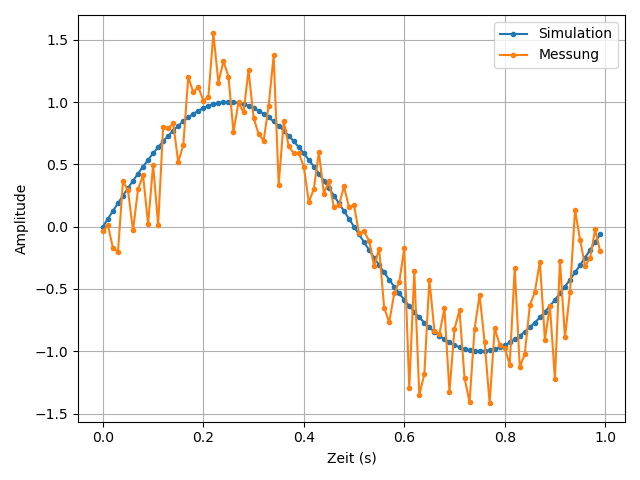
\includegraphics[width=8cm,align=t]{pics/Matplotlib/SimpleExample.png}
\end{minipage}
%%%%%%%%%%%%%%%%%%%%%%%%%%%%%%%%%%%%%%%%%%%%%%%%%%
\\[0.3cm]
%%%%%%%%%%%%%%%%%%%%%%%%%%%%%%%%%%%%%%%%%%%%%%%%%%
\textbf{OOP Beispiel}
\\
\begin{minipage}[h]{10cm}
	\lstinputlisting{code/Matplotlib/OOP_Beispiel.py}
\end{minipage}
\begin{minipage}[h]{8cm}
	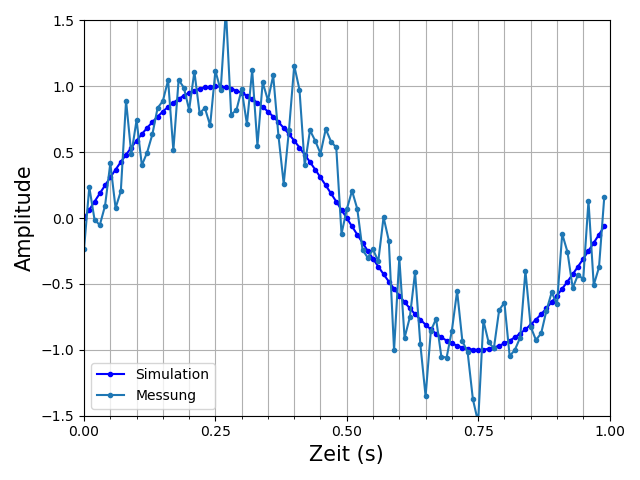
\includegraphics[width=8cm,align=t]{pics/Matplotlib/OOP_Beispiel.png}
\end{minipage}
%%%%%%%%%%%%%%%%%%%%%%%%%%%%%%%%%%%%%%%%%%%%%%%%%%
\newpage
%%%%%%%%%%%%%%%%%%%%%%%%%%%%%%%%%%%%%%%%%%%%%%%%%%
\textbf{Subplots}
\\
\begin{minipage}[h]{10cm}
	\lstinputlisting{code/Matplotlib/Subplots.py}
\end{minipage}
\begin{minipage}[h]{8cm}
	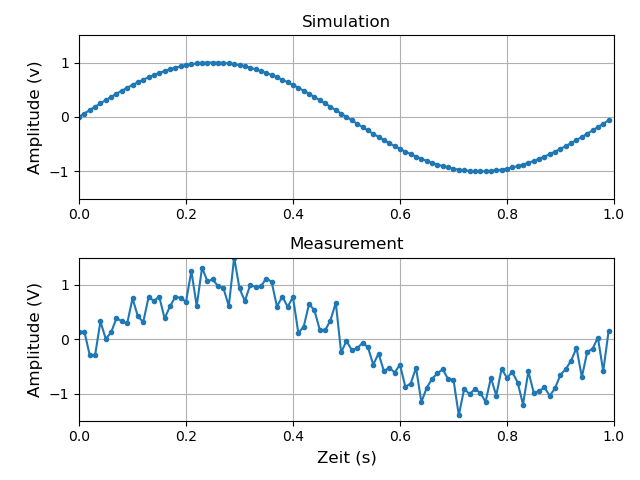
\includegraphics[width=8cm,align=t]{pics/Matplotlib/Subplots.png}
	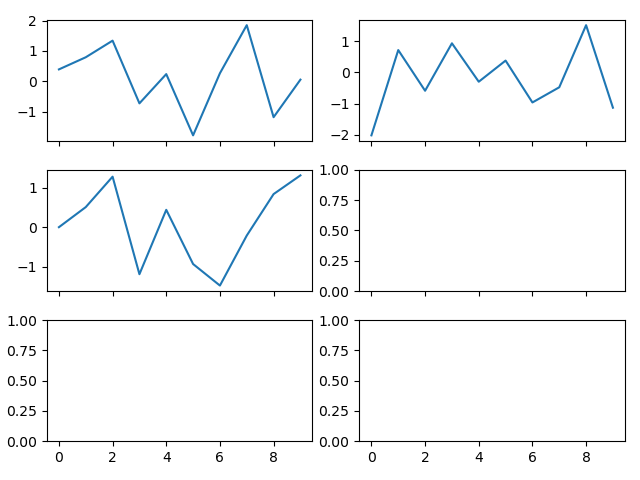
\includegraphics[width=8cm,align=t]{pics/Matplotlib/MultSubplots.png}
\end{minipage}
%%%%%%%%%%%%%%%%%%%%%%%%%%%%%%%%%%%%%%%%%%%%%%%%%%
\newpage
%%%%%%%%%%%%%%%%%%%%%%%%%%%%%%%%%%%%%%%%%%%%%%%%%%
\textbf{logarithmische Darstellung}
\\
\begin{minipage}[h]{10cm}
	\lstinputlisting{code/Matplotlib/Log.py}
\end{minipage}
\begin{minipage}[h]{8cm}
	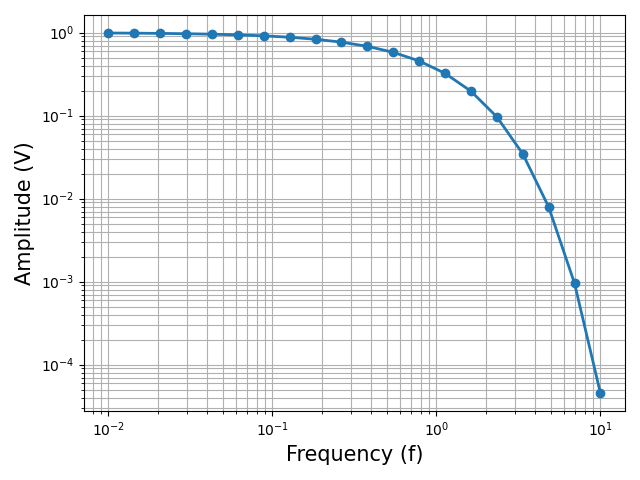
\includegraphics[width=8cm,align=t]{pics/Matplotlib/Loglog.png}
	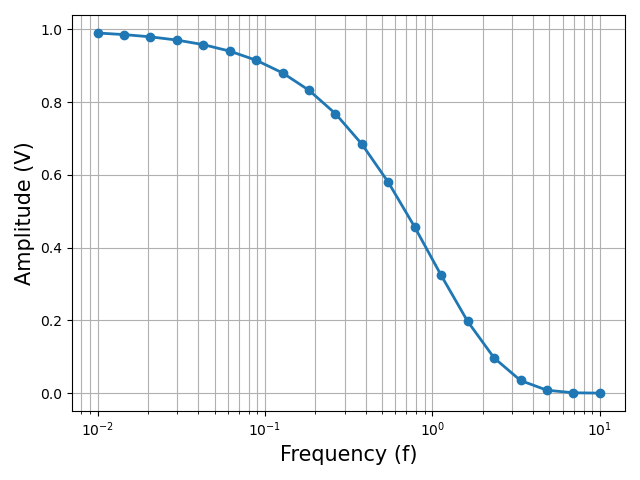
\includegraphics[width=8cm,align=t]{pics/Matplotlib/Semilogx.png}
\end{minipage}
%%%%%%%%%%%%%%%%%%%%%%%%%%%%%%%%%%%%%%%%%%%%%%%%%%